%******************************************************************
% Proyecto de Título                                              *
% Ingeniería Civil en Informática - Universidad Austral de Chile  *
% Autor: Paulo Antonio Gallardo Casanova                          *
%          gallardo.casanova@gmail.com                            * 
% Tesis: Uso de 6LoWPAN para el Monitoreo de la Salud             *
%            Estructural de un Puente                             *
%     Noviembre de 2013 - Valdivia                                *   
% Patrocinante: Christian Lazo, clazo@inf.uach.cl                 *                                         
%******************************************************************

%******************************************************************
% Plantilla de Proyecto de Título                                 *
% Ingeniería Civil en Informática - Universidad Austral de Chile  *
% Autor: Paulo Antonio Gallardo Casanova                          *
%          gallardo.casanova@gmail.com                            * 
%     Agosto de 2013 - Valdivia                                   *                                            
%******************************************************************

%******************************************************************
% Proyecto de Título                                              *
% Ingeniería Civil en Informática - Universidad Austral de Chile  *
% Autor: Enzo Edgardo Vera Paganrd                                *
%          eevp88@gmail.com                                       * 
%     Enero 2014 - Valdivia                                       *
%******************************************************************
\documentclass[12pt]{article} 
\usepackage[papersize={216mm,330mm},left=4cm,right=2.5cm,top=1.88cm,bottom=3cm]{geometry} 
\usepackage[spanish]{babel}
\usepackage[utf8]{inputenc}
\usepackage{graphicx}
\usepackage{xcolor}
\usepackage{xcolor,colortbl}
\usepackage[pdftex,
			colorlinks=true,
			linkcolor=black,
			citecolor=black,
			filecolor=black,
			urlcolor=black,
			hyperfootnotes=false,
            pdfauthor={Enzo Edgardo Vera Pagnard},
            pdftitle={Dispositivo identificador de personas con RFID y Biometria},
            pdfsubject={Tesis},
            pdfkeywords={DIPRB, RFID},
            pdfproducer={Latex with hyperref},
            pdfcreator={pdflatex}]{hyperref}
\usepackage{url}
\usepackage[bottom]{footmisc}
\usepackage{float}
\usepackage{nonfloat}
\usepackage{setspace}
\usepackage[titles]{tocloft}
\usepackage{lipsum,titletoc}
\usepackage{tocloft}
\usepackage{amsmath}
\usepackage[T1]{fontenc} % Times New Roman
\usepackage{txfonts}
\usepackage{sectsty}
\usepackage[labelsep=period]{caption}
\usepackage{multirow}
\usepackage{fancyhdr}
\pagestyle{fancy}
\fancyhead{}
\fancyfoot[CE,CO]{\thepage}
\renewcommand{\headrulewidth}{0.0pt}
\renewcommand{\footrulewidth}{0.0pt}
\usepackage[figuresright]{rotating} 
\renewcommand{\baselinestretch}{1.5}
\pretolerance=10000
\tolerance=10000

\sectionfont{\fontsize{14}{14}\selectfont}
\subsectionfont{\fontsize{14}{14}\selectfont}

\newcommand{\blockline}{\par\noindent\hspace{-0.05\textwidth}%
    \textcolor{black}{\rule{1.05\textwidth}{0.35mm}}\par\nobreak}
       
    
\begin{document}

%##########################################################
%PORTADA

\thispagestyle{empty}
\setcounter{page}{1}
\begin{spacing}{1.0}

\begin{center}

\includegraphics[width=2.65cm, height=3.18cm]{images/portada/escudo.png}\\
\vspace{0.5cm}

\includegraphics[width=13.02cm, height=1.23cm]{images/portada/uach.png}\\
\vspace{-0.4cm}
\blockline
\vspace{0.2cm}
{\fontsize{24}{24}\selectfont Facultad de Ciencias de la Ingeniería}\\[0.1cm]
{\fontsize{18}{18}\selectfont Escuela de Ingeniería Civil en Informática}\\
\end{center}

\vspace{3.0cm}

\begin{center}
{\fontsize{18}{18}\selectfont \bf DISPOCITIVO IDENTIFICADOR DE PERSONAS CON RFID Y BIOMETRÍA}\\[0.5cm]
{\fontsize{18}{18}\selectfont \bf DIPRB}\\
\end{center}

\vspace{3.0cm}

\begin{flushright} \small
{\fontsize{10}{10}\selectfont Proyecto para optar al título de}  \textcolor{white}{.}\\
{\fontsize{10}{10}\selectfont \bf Ingeniero Civil en Informática} 
\end{flushright}

\vspace{1.0cm}

\begin{flushleft} \small
\hspace{-1cm}{\fontsize{11}{11}\selectfont PROFESOR PATROCINANTE:}\\
\hspace{-1cm}{\fontsize{11}{11}\selectfont NOMBRE DEL PATROCINANTE}\\
\hspace{-1cm}{\fontsize{11}{11}\selectfont TÍTULOS Y GRADOS DEL PATROCINANTE}\\
\vspace{0.5cm}
\hspace{-1cm}{\fontsize{11}{11}\selectfont PROFESOR CO-PATROCINANTE:}\\
\hspace{-1cm}{\fontsize{11}{11}\selectfont NOMBRE DEL CO-PATROCINANTE}\\
\hspace{-1cm}{\fontsize{11}{11}\selectfont TÍTULOS Y GRADOS DEL CO-PATROCINANTE}\\
\vspace{0.5cm}
\hspace{-1cm}{\fontsize{11}{11}\selectfont PROFESOR INFORMANTE:}\\
\hspace{-1cm}{\fontsize{11}{11}\selectfont NOMBRE DEL INFORMANTE}\\
\hspace{-1cm}{\fontsize{11}{11}\selectfont TÍTULOS Y GRADOS DEL INFORMANTE}\\
\end{flushleft}

\vspace{1.0cm}

\begin{center}
{\fontsize{16}{16}\selectfont \bf ENZO EDGARDO VERA PAGNARD}\\
\vspace{0.4cm}
{\fontsize{10}{10}\selectfont VALDIVIA - CHILE}\\
{\fontsize{10}{10}\selectfont 2014}\\
\end{center}

\end{spacing}

%##########################################################

\newpage

\newgeometry{left=4cm,right=2.5cm,top=4cm,bottom=3cm} % Márgenes documento
\renewcommand{\tablename}{Tabla}

% Formato de indices
\renewcommand\contentsname{}
\renewcommand\listfigurename{}
\renewcommand\listtablename{}

\setlength{\cftbeforesecskip}{0ex}
\titlecontents{section} 
[2.3em]                 
{\rmfamily}            
{ \contentslabel{1.3em}} 
{\hspace*{-1.0em}}
{\titlerule*[0.7pc]{.}\contentspage}

\setlength{\cftsecnumwidth}{0.8em}  % espacio en ToC
\setlength{\cftsubsecnumwidth}{1.8em}
\setlength{\cftsubsubsecnumwidth}{2.5em}
\setlength{\cftsubsecindent}{2.0em}
\setlength{\cftsubsubsecindent}{3.0em}
\setlength{\cftfignumwidth}{1.5em}  % espacio entre números con LoF
\setlength{\cfttabnumwidth}{1.5em}  % espacio entre números con LoT


\setlength{\parindent}{0pt} % sangrías

%----------------------------------------------------------
% NOTAS

%----------------------------------------------------------
% AGRADECIMIENTOS
\thispagestyle{empty}
\begin{center}
{\fontsize{14}{14}\selectfont \bf AGRADECIMIENTOS}\\
\end{center}

%\input{contents/Agradecimientos.tex}

\newpage

\setcounter{page}{1}
\renewcommand{\thepage}{\roman{page}} 

%##########################################################
%INDICES

%----------------------------------------------------------
% Indice de contenidos
\begin{center}
{\fontsize{14}{14}\selectfont \bf ÍNDICE}\\
\end{center}
\phantomsection
\addcontentsline{toc}{section}{ÍNDICE}
\vspace{-1.0cm}
\begin{spacing}{1.2}
{\fontsize{10}{10}\selectfont \tableofcontents}
\end{spacing}

\newpage

%----------------------------------------------------------
% Indice de tablas - LoT
\begin{center}
{\fontsize{14}{14}\selectfont \bf ÍNDICE DE TABLAS}\\
\end{center}
\phantomsection
\addcontentsline{toc}{section}{ÍNDICE DE TABLAS}

\begin{flushright} \small
TABLA \hspace{11.6cm} PÁGINA\\
\end{flushright}

\vspace{-1.0cm}

\begin{spacing}{1.2}
{\fontsize{10}{10}\selectfont \listoftables}
\end{spacing}

\newpage

%----------------------------------------------------------
% Indice de figuras - LoF
\begin{center}
{\fontsize{14}{14}\selectfont \bf ÍNDICE DE FIGURAS}\\
\end{center}
\phantomsection
\addcontentsline{toc}{section}{ÍNDICE DE FIGURAS}


\begin{flushright} \small
FIGURA \hspace{11.45cm} PÁGINA\\
\end{flushright}

\vspace{-1.0cm}

\begin{spacing}{1.2}
{\fontsize{10}{10}\selectfont \listoffigures}
\end{spacing}

\newpage


%----------------------------------------------------------
% RESUMEN
\begin{center}
{\fontsize{14}{14}\selectfont \bf RESUMEN}\\
\end{center}
\phantomsection
\addcontentsline{toc}{section}{RESUMEN}

%----------------------------------------------------------
%----------------------------------------------------------
% RESUMEN

\vspace{0.5cm}




%----------------------------------------------------------
%----------------------------------------------------------


\newpage

%----------------------------------------------------------
% ABSTRACT
\begin{center}
{\fontsize{14}{14}\selectfont \bf ABSTRACT}\\
\end{center}
\phantomsection
\addcontentsline{toc}{section}{ABSTRACT}

%%----------------------------------------------------------
%----------------------------------------------------------
% ABSTRACT

\vspace{0.5cm}

Today, the technological devices are increasing and they are being incorporated in daily life. The technological devices give to us an unusual degree of connectivity, for example: tablets, smartphones, or even everyday things, such as a refrigerator. In this context, the humanity begins to live with a network of interconnected devices that is known as the ``Internet of Things'', which will be the next technological revolution, bringing new opportunities and challenges for the users, business and society. In this scenario, the objective of this project is to communicate devices through 6LoWPAN, a standard based on the IPv6 protocol over low-power and lossy networks to support the Internet of Things, using open hardware platforms and emphasizing the singularities of embedded systems, such as a limited number of operations, low power consumption and low band width capability. In addition, the prototype uses the standard 6LoWPAN in a network environment that brings the Internet of Things to a Bridge Management System for optimizing maintenance of structures.\\


%----------------------------------------------------------
%----------------------------------------------------------

\newpage

%##########################################################
% CUERPO DEL DOCUMENTO

\setcounter{page}{1}
\renewcommand{\thepage}{\arabic{page}}

%----------------------------------------------------------
%----------------------------------------------------------
\section{INTRODUCCIÓN}
%----------------------------------------------------------
%----------------------------------------------------------
% INTRODUCCIÓN

En la búsqueda de soluciones más eficientes y a bajo costo, conocer de componentes electrónicos como sensores (luminosidad, humedad, temperatura, etc.), microcontroladores, servo motores, pantallas LCD, entre otros, son herramientas poderosas debido a las diferentes problemáticas que pueden dar solución, integrar estas tecnologías dan un gran valor agregado a cualquier tipo proyecto, permitiendo solucionar en el ambiente del usuario diferentes problemáticas de manera útil y efectiva.

Para lograr que este dispositivo interactúe con el ambiente donde está inmerso y se comunique con una base de datos de manera local o de forma remota a través de Internet se hace necesario el desarrollo de piezas de software, capaz de procesar la información recolectada, ya sea en tiempo real o cuando sea necesario, dando de esta manera las funcionalidades necesaria para cubrir las necesidades demandadas.

Para realizar este proyecto se utilizara plataformas de Open Hardware, lo que nos brinda la libertada de construir un dispositivo capaz integrar cualquier tipo de sensor estándar, lo cual nos permite generar el conocimiento para manipular cualquier tipo de sensor.

%--------------------------------------

%--------------------------------------

%--------------------------------------

%--------------------------------------
\subsection{Objetivos}

%-----------------------
\subsubsection{Objetivo general}

Construir un dispositivo capas de cuantificar y controlar el flujo de personas de algún espacio físico y con esto gestionar su mantención de mejor manera. El dispositivo debe ser capaz de integrar distintos sensores de reconocimientos (RFID y lector biométrico), comunicarse con un servidor para poder guardar la información en una base de datos y generar algunos reportes.
\vspace{-0.4cm}
%-----------------------
\subsubsection{Objetivos específicos}


\begin{enumerate}
\item Estudiar las diferentes tecnologías de Open Hardware relevantes para este proyecto, incluyendo sensores (RFID y lector biométrico) y microcontrolador.
\item Definir arquitectura del sistema que permita la escalabilidad e integración con otros sistemas, definiendo estándares de comunicación entre otros.
\item Seleccionar la plataforma de Open Hardware y sensores atingentes al proyecto, diseñar piezas de software que permita comunicar el dispositivo con la base de datos.
\item Modelar e implementar la base de datos que permita manipular la información eficientemente.
\item Entender nuevas tecnologías de programación web para implementar un prototipo de software de administrador de espacios.
\item Realizar pruebas evaluación del funcionamiento del sistema.
\end{enumerate}

\vspace{0.5cm}

%--------------------------------------
\subsection{Motivación}
El desarrollar conocimiento de plataformas de Open Hardware, tanto desde el punto de vista de la electrónica, como de metodologías de desarrollo de software, si bien las metodologías de desarrollo de software tradicionales no son las más adecuadas para este tipo de plataformas, es importante explorar como adaptar está metodologías a este tipo de proyectos.

Una de las áreas donde existe una brecha considerable en la formación como estudiantes, es en la solución de problemas en industrias manufactureras, no desde el punto de vista de la gestión o administración, sino en cubrir funcionalidades prácticas que presenten problemas dentro de los procesos productivos, como por ejemplo detener un motor si la temperatura de él es mayor a 100 grados Celsius o detener una prensa hidráulica si ocurre algún improvisto en la línea de producción, esta área sea transformado en un mercado creciente dentro de este tipo de industria\cite{Ind09} y representa un potencial nicho de mercada para futuros emprendimientos en el área de tecnologías de información y comunicación.

Además poder realizar algunas estadísticas sobre estas máquinas, ayudando a la gestión de estás misma, contribuyendo a los objetivos estratégicos del cliente, con este proyecto en algún grado se acortará esta brecha obteniendo datos del ambiente para luego procesarlos y
automatizar procesos.
\newpage
\subsection{Impacto}

Como este proyecto estará desarrollado en plataformas de Open Hardware y Open Software generará una base de conocimiento con respecto a la integración de dispositivos electrónicos a motores de bases de datos y plataformas web para manejar esta información, ahorrando tiempo y dinero, si en algún momento se requiere de este conocimiento para realizar algún producto de TIC que necesite manejar variables del ambiente en donde se encuentran inmersos y controlar otros dispositivos.

%----------------------------------------------------------
%----------------------------------------------------------


\newpage
%----------------------------------------------------------
%----------------------------------------------------------
\section{MARCO TEÓRICO}
%----------------------------------------------------------
%----------------------------------------------------------
% MARCO TEÓRICO

A lo largo del presente capítulo se pretende describir los conceptos en torno a los cuales se efectuará el siguiente trabajo. Además se llevará a cabo una revisión de las  tecnologias relacionadas con este proyecto como  son las  plataformas open hardware, sensores y microcontroladores .

%--------------------------------------
\subsection{Open Hardware}
\subsubsection{¿Qué es Open Hardware?}
Se les llama Open Hardware a todos los dispositivos de hardware cuyas especificaciones y diagramas esquemáticos son de acceso público, ya sea bajo algún tipo de pago o de forma gratuita. Algo que tienen en común el Open Hardware y el Open Software es que ambos corresponden a las partes tangibles de un sistema informático.

El Open Software ofrece al usuario cuatro libertades de uso, de estudio  y modificación, de  distribución y de redistribución de las versiones modificadas. Existen licencias que  garantizan y dan cobertura legal,  como  por  ejemplo  la  licencia  GNU GPL. El Open Hardware toma es mismas ideas del Open Software para aplicarlas en su campo.\cite{Osh14}

Esta idea es tan antigua  como la  del Open Software, sin embargo  su  empleo no es tan directo compartir  diseños  de  hardware  es  un poco  más  complicado no se cuenta  con una definición exacta. Incluso Richard Stallman Presidente de la  Free Software Foundation afirma  que  las  ideas del Open Software  se  pueden  aplicar  a los archivos  o fichero necesarios  para el diseño y especificación, pero no  al circuito físico  en  sí.  

Al no existir una  definición clara de Open Software cada persona  lo  interpreta  a su manera. Dependiendo  del  enfoque  pueden  ser  establecidas dos clasificaciones  la primera  tiene en cuenta  cómo es  su naturaleza estático o  reconfigurable  y la  otra   en función  de  su filosofía.

\myparagraph{Según su Naturaleza}

Dada su diferente naturaleza, al hablar de Open hardware hay que especificar de qué tipo de hardware se está hablando. A continuación se describen cada uno de los diferentes hardwares según su naturaleza:

\begin{itemize}
\item \textbf{Hardware reconfigurables}\\
Es aquél descrito mediante un lenguaje de descripción de hardware. Su naturaleza es completamente diferente a la del hardware estático. Se desarrolla de una manera muy similar a como se hace con el software, mediante archivos de texto, que contienen el código fuente. Se les puede aplicar directamente una licencia libre, como la GPL. Los problemas no surgen por la definición de qué es libre o qué debe cumplir para serlo, sino que aparecen con las herramientas de desarrollo necesarias. Para hacer que el hardware reconfigurable sea libre, sólo hay que aplicar la licencia GPL a su código.\\
\item \textbf{Hardware estático}\\
Es el conjunto de elementos materiales o tangibles de los sistemas electrónicos.
\end{itemize}

\myparagraph{Según su filosofía}

Al no existir una definición clara de Open Hardware, también existe libertad en su interpretación. Muchos de los argumentos acerca del diseño de Open Hardware provienen de quienes hablan en las comunidades de software y hardware. Una causa de esto es el simple hecho de que la palabra ``software'' refiere tanto al código fuente como a los archivos o ficheros ejecutables, mientras que las palabras ``hardware'' y ``diseño de hardware'' se refieren claramente a dos cosas distintas. Usar la palabra ``hardware'' como taquigrafía para el diseño y el objeto físico es una receta para la confusión. Los términos siguientes se han utilizado en discusiones de este asunto.

\begin{itemize}
\item \textbf{Free hardware design}\\
Se refiere a un diseño que pueda ser copiado, distribuido, modificado, y fabricado libremente. No implica que el diseño no pueda también ser vendido, o que cualquier puesta en práctica de hardware del diseño estará libre de coste. Todas las mismas discusiones sobre el significado de la ``libertad'' entre los partidarios de la \emph{Free Software Foundation}, y los partidarios de la Licencia BSD que afecta al software, desafortunadamente las trasladan a los diseños del hardware.\\
\item \textbf{Open source hardware}\\
Se refiere al hardware para el cual toda la información del diseño se pone a disposición del público en general. Open source hardware se puede basar en un free hardware design, o el diseño en el cual se basa puede ser restringido de alguna manera.\\
\item \textbf{Open Hardware}\\
Es una marca registrada del Open Hardware Specification Program. Es una forma limitada de open source hardware, para la cual el requisito es que: La suficiente documentación del dispositivo debe estar disponible para que un programador competente pueda escribir un controlador del dispositivo. La documentación debe cubrir todas las características de la interfaz del dispositivo - controlador que se espera que cualquier usuario emplee. Esto incluye funciones de entrada-salida, de control y funciones auxiliares como medidas de funcionamiento o diagnósticos de auto prueba. Los detalles de soporte de firmware on-board y de la puesta en práctica de hardware no necesitan ser divulgados excepto cuando son necesarios para permitir programar un controlador para el dispositivo.\cite{Del07}

Es decir, solamente una cantidad de información limitada sobre el diseño necesita estar disponible; posiblemente no mucha, por ejemplo, para hacer una reparación.

\end{itemize}




%--------------------------------------
\subsection{Biometría}

Históricamente, la identificación personal se ha basado en posesiones especiales (llaves, tarjetas) o en conocimientos secretos (palabras claves, números de identificación personal), todos estos aspectos son casi únicos, y se emplean para verificar la identidad de su portador. Ahora bien, el ser humano posee características propias que lo hacen único: huellas dactilares, la voz, el rostro, la forma de escritura, e incluso el iris del ojo.Entonces, podemos decir que nosotros llevamos nuestras propias palabras claves, tarjetas o números PIN. Entonces, ¿Porque no aprovechar estas características?

Los científicos se formularon está misma pregunta hace algunos años, dando
origen a la Biometría. Ésta consiste en la identificación o verificación de la identidad de un individuo, empleando sus características biológicas, psicológicas y de conducta. En la actualidad, existen distintos tipos de dispositivos que soportan la biometría, tales como
lectores de huella digital o lectores de retina.\cite{Car08}
\newpage

Por definición, un sistema biométrico, es un sistema automático capaz de:

\begin{enumerate}

\item Obtener la muestra biométrica del usuario final.
\item Extraer los datos de la muestra.
\item Comparar los datos obtenidos con los existentes en la base de datos.
\item Decidir la correspondencia de datos.
\item Indicar el resultado de la verificación.
\end{enumerate}

Algunos de los dominios para esta tecnologia son:
\begin{itemize}
\item \textbf{Bioinformática}: Aplicación de la informática en el área de la medicina y la biología.
\item \textbf{Biometría forense}: La ciencia y tecnología de usar e interpretar la evidencia física para propósitos legales.
\item \textbf{Interacción Humano-Computador \textit{(Human-to-Computer Interaction-HCI)}}: Su objetivo es mejorar el rendimiento y la precisión de esas interfaces, mediante el reconocimiento de los usuarios y adaptarse a las características específicas de cada usuario para labores de reconocimiento.
\item \textbf{Seguridad biométrica}: Autenticación de usuarios. Enlazar la información digital a una determinada identidad para lograr control de acceso, autenticación de información entre otras.
\end{itemize}

En  este  trabajo de  titulación,este  último dominio es el  que nos interesa y  en el  cual  se  centraremos especial  atención y esfuerzos.

Cabe destacar que todos los métodos biométricos conocidos son ``no determinísticos'' y necesitan estar basadas en aproximaciones heurísticas.

Existen 2 modos de operación en los sistemas de autenticación biométrica: El enrolamiento (\textit{Enrollment}) y la autentificación (\textit{Authentication}).

\subsubsection{Enrrolamiento y Autenticación}


Existen 2 modos de operación en los sistemas de autenticación biométrica: El enrolamiento (\textit{Enrollment}) y la autentificación (\textit{Authentication}).


\subsubsection*{Enrolamiento}

El proceso de enrolamiento ocurre cuando nos registramos en el sistema, donde las características de cada usuario se almacenan para futuras referencias y asociaciones de identidad de los sujetos. Una representación gráfica de este modo se aprecia en la Figura \ref{enrrolamiento}

\begin{figure}[H]
\centering
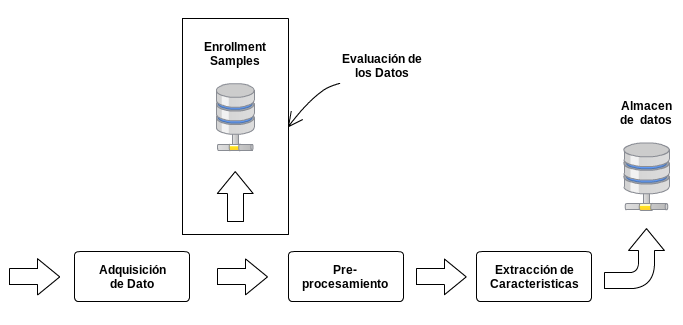
\includegraphics[scale=0.5]{images/capitulo2/enrrolamiento.png}
\caption{Esquema gráfico del proceso  de Enrrolamiento}
\label{enrrolamiento}
\end{figure}

Aquí se observa que el proceso comienza con la toma de datos (por ejemplo, medir y realizar conversiones análogo-digital). La representación digital posterior a este proceso es denominada Enrollment Samples(Ejemplos de Enrolamiento) o simplemente enrollments. Desde el enrollment original se extraen las características biométricas, son preprocesadas, y en algunos casos almacenadas en algún soporte de datos (como una base de datos) para poder reproducirlas en otro momento.

\myparagraph{Autenticación}

La Autenticación (\textit{authetication}) consiste en el proceso de verificar o identificar la identidad de algún sujeto, según corresponda,  en la Figura \ref{autenticacion} se muestra en forma gráfica este proceso.

\begin{figure}[H]
\centering
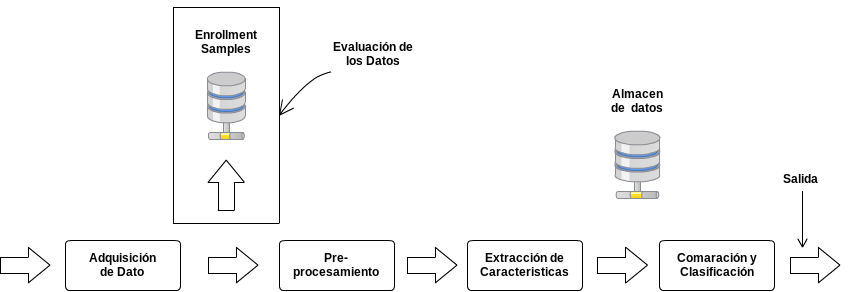
\includegraphics[scale=0.5]{images/capitulo2/autenticacion.png}
\caption{Esquema gráfico del proceso  de Autenticación}
\label{autenticacion}
\end{figure}


\subsubsection{Verificación versus Identificación}

La autenticación la podemos dividir en dos acciones verificación y identificación, en función de cómo se desee obtener la identidad del sujeto.

\myparagraph{Verificación}
El modo de Verificación es el sistema de autentificación que determina si un set determinado de características son similares al template de dicha persona para determinar si es o no es la persona. El resultado de esta acción es siempre una decisión binaria(si o no, 0 o 1) entregando en algunos casos el puntaje de acierto (Matching Score), lo que muestra el grado de similitud entre su template y ésta persona.

\myparagraph{Identificación}

El modo de Identificación describe el proceso de determinar la identidad de un sujeto (dadas sus características biométricas) comparándolas con un rango de sujetos. Así, la clasificación asignada será una entre todas las personas registradas en el sistema.



Para ejemplificar estos conceptos, veamos los siguientes ejemplos.

\begin{itemize}

\item Si tenemos un control de acceso para un portal principal, nuestro problema es ``Determinar quién es'', para en función de eso, determinar si ingresa o no. Esto sería una identificación.

\item Si tenemos una oficina del usuario ``Pedro Paredes'', donde sólo él tiene asignado acceso, nuestro problema es ``Determinar si soy Pedro Paredes'', por lo tanto, verificar si soy el usuario determinado. Esto es una verificación.
\end{itemize}

Es fundamental entender ambos mecanismos y encontrar el más adecuado para nuestros requerimientos.

\subsubsection{Criterios de selección de características biométricas}

Se han sugerido distintos criterios para autenticar de manera adecuada. A continuación veremos los 4 más importante:
\begin{enumerate}
\item \textbf{La Variabilidad} La Variabilidad tiene que ver con la variación de los valores desde un evento a otro, sobre una misma persona. Este efecto es llamado variabilidad Intra-Personal o Intra-Class. La variabilidad es inherente a todos los sistemas biométricos debido a la naturaleza no determinística de las mediciones biométricas, en la Figura \ref{la_variabilidad} vemos un ejemplo de variabilidad  \cite{Way00}.

\begin{figure}[H]
\centering
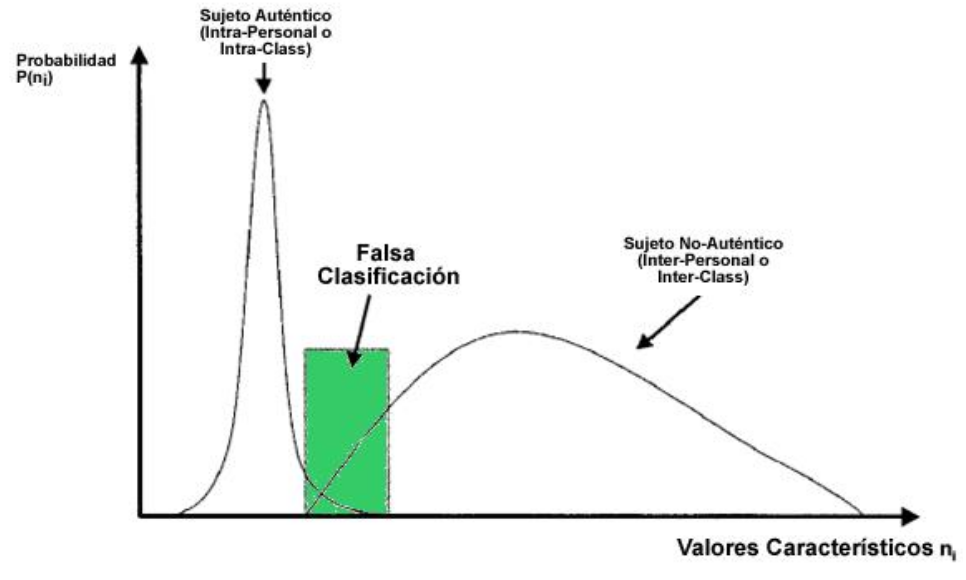
\includegraphics[scale=0.3]{images/capitulo2/la_variabilidad.png}
\caption{Ejemplo de variabilidad y capacidad de discriminar una característica biométrica}
\label{la_variabilidad}
\end{figure}


\item \textbf{La Capacidad Discriminatoria}  está determinada por el grado de unicidad de las características biométricas que serán utilizadas en la comparación. Aparentemente, un buen sistema biométrico posee una baja variabilidad Intra-Personal y una alta variabilidad Inter-Personal (entre distintas personas). El grado de variabilidad Intra-Personal está reflejado por el ancho de una distribución gaussiana (ver Figura \ref{la_variabilidad}) para sujetos auténticos, donde la capacidad discriminatoria puede ser estimada en la intersección de las curvas de sujetos auténticos versus sujetos no-auténticos \cite{Zha00}.

\item \textbf{La Acertividad}, para diseñar un sistema biométrico funcional, las características deben poseer bastante acertabilidad en un tiempo aceptable. Hoy en día, el criterio es determinado por la tecnología del sensor, planteando la inquietud de saber si obtuvo la característica en un tiempo aceptable y con la suficiente calidad. Por ejemplo, un examen de ADN es muy exacto, sin embargo, requiere un amplio tiempo de trabajo de verificación \cite{Zha00}.


\item \textbf{El Rendimiento}, cuando nos referimos a que una característica biométrica debe ser procesada en un tiempo aceptable nos referimos al rendimiento de un sistema biométrico.  de una persona para el ingreso a una oficina. Por lo general asociamos el grado de exactitud en función del tiempo de respuesta que deseemos obtener \cite{Way00}.

\end{enumerate}


\subsubsection{Medidas de Rendimiento y Exactitud}

Los sistemas biométricos intentan determinar o verificar la identidad de cada miembro registrado en nuestro sistema utilizando medidas y/o características distintivas. Debido a la naturaleza no-determinística de este proceso, es imposible realizar un análisis exacto (con los sistemas del día de hoy). Evaluaciones técnicas sugieren que éstas deben ser realizadas mediante análisis estadísticos y mediciones empíricas.

Según el tipo de medición biométrica que deseemos utilizar, se utilizan distintos indicadores. A través de las últimas 2 décadas, se llegó al consenso en cuáles eran las mediciones más importantes, para realizar las evaluaciones técnicas pertinentes \cite{Way99} y que son presentadas en la tabla \ref{tabla_medidas}.



\begin{spacing}{1.0}
\begin{table}[H]
\centering
\caption{Pricipales medidas para evaluaciones de los sistemas biométricos} 
\begin{tabular}{|c|c|}
\hline 
\rowcolor{green!50} &\\
\rowcolor{green!50} \textbf{Medida} & \textbf{Descripción}\\[0.3cm]
\hline 
\textbf{Tasa de Falsos Aciertos} &\makebox[8.5cm][l]{Tasa entre coincidencias detectadas por el sistema}\\
\textit{False Match Rate} (FMR)  &\makebox[8.5cm][l]{pero que no son reales (falsos positivos) versus el}\\
\textit{False Accept Rate} (FAR) &\makebox[8.5cm][l]{número total de muestras.}                           \\
\hline
\textbf{Tasa de Falso Rechazo} &\makebox[8,5cm][l]{Tasa entre coincidencias que no son detectadas}\\
\textit{False Non-Match Rate (FNMR)} & \makebox[8,5cm][l]{por el sistema pero que sí son reales (falsos}\\
\textit{False Reject Rate (FRR)} & \makebox[8,5 cm][l]{negativos) versus el número total de muestras.}\\
\hline
\textbf{Tasa donde los errores son iguales} & \makebox[8,5cm][l]{El punto en el diagrama de tasa de errores donde}\\
\textit{Equal-Error-Rate (EER)} & \makebox[8,5cm][l]{las tasa de falsos aciertos es igual a la tasa de}\\
 & \makebox[8,5cm][l]{falsos rechazos.} \\
\hline
\textbf{Tasa de error por particionamiento} & \makebox[8,5cm][l]{Tasa de falsos rechazos debido a errores de}\\
\textit{Binning Error Rate (BNR)} & \makebox[8,5cm][l]{particionamiento.}\\
\hline
\textbf{Coeficiente de Penetración} & \makebox[8,5cm][l]{Porcentaje promedio del tamaño del repositorio}\\
\textit{Penetration Coefficient (PC)} & \makebox[8,5cm][l]{de datos a ser revisado para cada proceso de} \\
 & \makebox[8,5cm][l]{autenticación.}\\
\hline
\textbf{Tiempo de Transacción} & \makebox[8,5cm][l]{Tiempo requerido para una sola transacción de}\\
\textit{Transaction Time (TT)} & \makebox[8,5cm][l]{autenticación, compuesto por la suma del tiempo}\\
 & \makebox[8,5cm][l]{de recolección de datos y el tiempo de cálculo.}\\
\hline

\end{tabular}
\label{tabla_medidas}
\end{table}
\end{spacing}

Las dos primeras medidas definen el umbral de decisión (\textit{threshold}) desde donde  se puede optimizar el nivel de exactitud en función del tiempo de búsqueda como  se muestra en la Figura\ref{umbral}. esto quiere decir que a un alto valor de umbral implica un sistema menos exacto, por lo  cual podria aceptar a quien no posee los permisos correspondientes, pero más rápido a la hora de entregar resultados. Por el contrario, con un bajo umbral de decisión, es menos probable equivocarse, pero el tiempo de procesamiento es mucho mayor. A pesar de la importancia de estos indicadores en los distintos dispositivos biométricos, no es objetivo de este proyecto de título entrar en mayores detalles.


\begin{figure}[H]
\centering
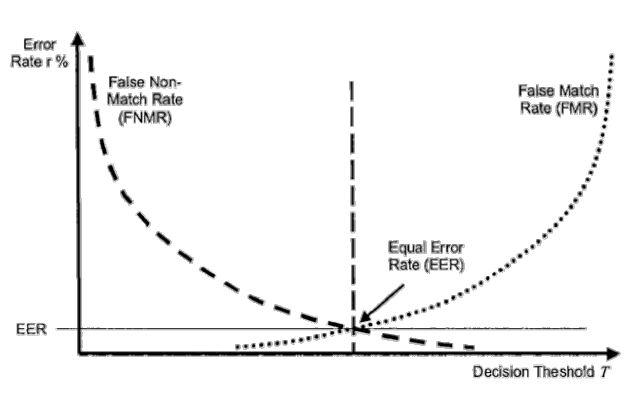
\includegraphics[scale=0.5]{images/capitulo2/umbral.png}
\caption{FNMR, FMR y EER en función del umbral de decisión}
\label{umbral}
\end{figure}

\subsubsection{Dactiloscopía: Reconocimiento de huellas dactilares}

La base de ésta modalidad biométrica es la estructura que posee la piel en la punta de los dedos. Se trata de una característica biológica fenotípica, es decir, una manifestación específica de determinados rasgos, que serían únicos, incluso en caso de personas que son gemelos.\\

La estructura biométrica está compuesta por ``crestas papilares'' y los ``surcos interpapilares'', comúnmente llamados ``crestas'' y ``valles''. Las crestas papilares son los relieves epidérmicos situados en la palma de las manos y en la planta de los pies, mientras que los surcos interpapilares se determinan por las depresiones que separan dichos relieves o crestas. Dentro de las crestas papilares existen los llamados ``poros papilares'', que son diminutos orificios de variadas formas y dimensiones por los cuales se expulsa el sudor. Una vez que el sudor sale al exterior, se derrama por todas las crestas y se mezcla con la grasa natural de la piel, dando lugar a que cuando se toque un objeto apto para la retención de huellas, éstas queden impresas en el mismo. Esta es la base de la impresión dactilar.


Se ha demostrado científicamente y comprobado por la experiencia, que son perennes, inmutables y diversiformes 



\begin{itemize}
\item\textbf{Son perennes}, porque desde que se forman en el sexto mes de la vida intrauterina, permanecen invariantes en número, situación, forma y dirección hasta la muerte, en que la putrefacción destruye la piel.
\item\textbf{Son inmutables}, ya que las crestas papilares no pueden modificarse   fisiológicamente. Si hay un traumatismo poco profundo, se regeneran y si es profundo, las crestas no reaparecen con forma distinta a la que tenían, sino que la parte afectada por el traumatismo resulta invadida por un dibujo cicatrizal.
\item\textbf{Son diversiformes}, pues no se ha hallado todavía dos impresiones idénticas producidas por dedos diferentes.
\end{itemize}


\myparagraph{Clasificación}

En la  actualidad, existen tres niveles de clasificación entre los cuáles es posible obtener imágenes de las huellas dactilares:

\begin{enumerate}
	\item \textbf{Características globales}: patrón de características definido a nivel mundial a partir de la colección de crestas existentes en un dedo, clasificado en dos clases de ``Wirbel'' (Whorl y doble ciclo) y cuatro clases de “lazos” \cite{Bal97}. La Figura \ref{clasifica} muestra un diagrama con la taxonomía respectiva.

\begin{figure}[H]
\centering
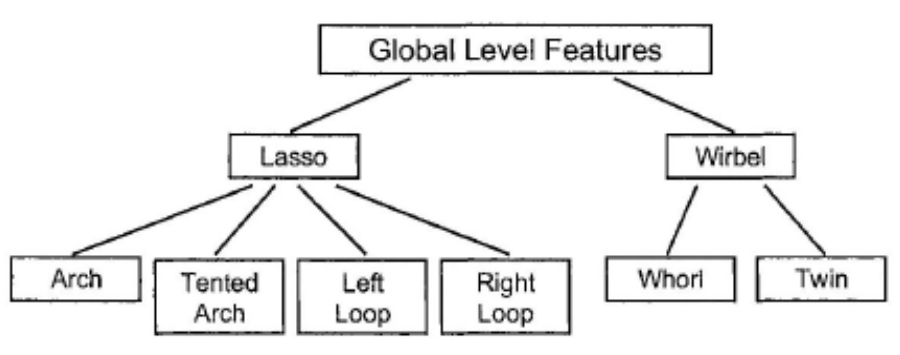
\includegraphics[scale= 0.45]{images/capitulo2/clasifica.png}
\caption{Clasificación de tres niveles de características globales de una huella dactilar}
\label{clasifica}
\end{figure}


\item\textbf{Características basadas en minucias}: estas  se basan en características e interrelaciones entre los distintos puntos, surcos y crestas dentro de un dominio espacial. La clasificación se origina a partir de elementos utilizados en medicina forense desde hace más de un siglo. Aquí se incluyen elementos tales como bifurcaciones, islas, terminaciones, empalmes, horquillas, lagos, cordilleras
independientes, entre otros.  En las Figuras \ref{minucias} y \ref{minucias2} se puede  observar algunos ejemlos de caracteristicas basadas en  minucias. 

\begin{figure}[H]
\centering
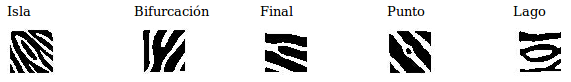
\includegraphics[scale= 0.8]{images/capitulo2/minucias.png}
\caption{Ejemplos de algunas características basadas en minucias}
\label{minucias}
\end{figure}



\begin{figure}[H]
\centering
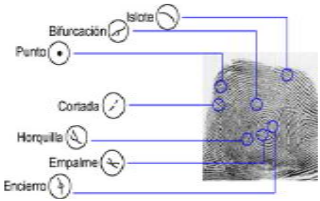
\includegraphics[scale= 0.8]{images/capitulo2/minucias2.png}
\caption{Ejemplo de  Huella digital y algunas características basadas en minucias}
\label{minucias2}
\end{figure}

\item\textbf{Características basadas en}: Los poros, aberturas de las glándulas sudoríparas, son visibles en la superficie del dedo y constituyen un patrón formado por los puntos en la cima de las crestas\cite{Rod97}. La adquisición de estas características, requieren de sensores de alta resolución espacial. En la figura \ref{poros_sudaderos} se muestra una ilustración de la distribución de éstas características.


\begin{figure}[H]
\centering
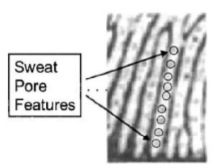
\includegraphics[scale= 0.8]{images/capitulo2/poros_sudaderos.png}
\caption{Ejemplo de  Huella digital y algunas características basadas en minucias}
\label{poros_sudaderos}
\end{figure}

\end{enumerate}

\myparagraph{Adquisición de los datos}

Para adquirir los datos de una huella dactilar se requieren dispositivos sensores específicos que puedan obtener una imagen de ella. Estos se puede dividir en sensores ópticos y sensores no ópticos. Los primeros requieren exponer la punta de los dedos a una superficie transparente que es sometida a la luz, observando su respuesta óptica; Los sensores no ópticos capturan la información sobre el perfil de altitud de la superficie de los dedos por medios distintos a la luz. Aquí se establece un voltaje eléctrico entre la piel y la superficie del sensor, que posee un conjunto de diminutos electrodos que generan voltaje cuando se expone a presión, obteniendo el perfil de alturas de las crestas y los valles. Existen otros sensores no ópticos que obtienen un perfil térmico de la piel de una distancia específica y que extraen la información de elevación desde un termograma bidimensional. En todos los casos, el resultado de la adquisición de los datos es un arreglo bidimensional de mediciones escalares que es habitualmente interpretado como imágenes en escalas de gris de distintas resoluciones y tamaños.

En las impresiones dactilares, los tamaños de imágenes generalmente se encuentran en el rango de $0.4$ a $1$ pulgada de altura y de $0.4$ a $0.6$ pulgadas de ancho, mientras que las resoluciones de escaneo de estos sensores se encuentran con valores entre $200$ a $1000$ dpi \cite{Mal03}.

\myparagraph{Extracción de Características}

Como se mencionó anteriormente, las características pueden ser clasificadas en 3 niveles: características globales, basadas en minucias y por el sudor de los poros. Aunque la primera y tercera categoría han mostrado una buena precisión en reconocimiento biométrico \cite{Bal97}, la mayoría de los enfoques se basan en la detección de minucias, no siendo ésta la excepción, por lo que se expondrá brevemente sobre las más comunes técnicas de procesamiento de imágenes para encontrar y clasificar los puntos característicos. Este procesamiento entrega un mapa de la ubicación espacial, la orientación y el tipo de características con respecto a la imagen original \cite{Rod97}.


La detección de minucias requiere numerosos pasos de preprocesamiento, que comienza con la utilización de filtros de mejoramiento de imagen tales como la ecualización de histogramas, para poner énfasis en las frecuencias relevantes en la imagen. Otro filtro que ha mostrado alta eficiencia es el filtrado basado en la dirección de la frecuencia, por ejemplo los filtros \emph{Gabor}, ya que pone énfasis en los cerros en una dirección local. Además, son aplicadas algunas rutinas estándares en el procesamiento de imágenes como lo son el suavizado, y el perfilado, seguido de un proceso de binarización para obtener imágenes reales en blanco y negro.


Basados en la imagen binaria, se aplican algoritmos de adelgazamiento y de erosión, que dan lugar a una imagen de representación en virtud de la representación de las crestas, que tendrán un ancho de $1$ pixel llamado ``esqueleto''. Un ejemplo de cómo va quedando la imagen con cada uno de estos procesos puede ser observado en la figura \ref{tratamiento}.


\begin{figure}[H]
\centering
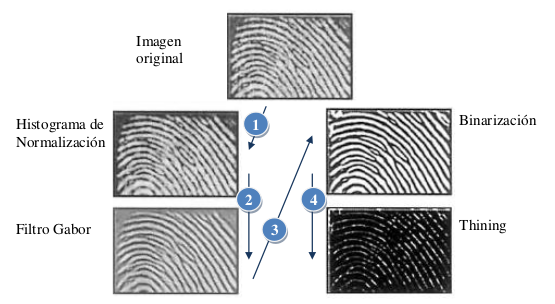
\includegraphics{images/capitulo2/tratamiento.png}
\caption{Tratamineto de imagen de una huella dactilar para encontrar puntos caracteristicos}
\label{tratamiento}
\end{figure}


Una vez obtenida las imágenes del esqueleto, la detección de las minucias es una tarea sencilla. Esto puede lograrse mediante de $8$ reglas de vecindad: cada pixel de la imagen es analizado en el contexto de sus $8$ pixeles vecinos. Un ejemplo es el caso que $1$ pixel tenga sólo $1$ vecino: este será clasificado como minucia terminal.


Note que detrás las técnicas basadas en minucias, existen otros tipos de características como crestas y características basadas en correlación, que requieren diferentes tipos de preprocesamiento. Particularmente, los métodos basados en correlación son sensibles a las transformaciones, por lo que requieren normalizaciones de tamaño y de orientación.


\myparagraph{Comparación y Clasificación}

La gran ventaja del reconocimiento de huellas dactilares basadas en minucias es la invariabilidad en escala y rotación de los puntos detectados. Esto quiere decir, que si rotamos o ampliamos la huella dactilar, los valores seguirán siendo los mismos, sin necesidad de hacer cálculos adicionales, razón por la que en vez de medir sus posiciones en términos de coordenadas absolutas o posición relativa, estas pueden compararse durante el proceso de correspondencia. Un ejemplo simplificado de esto es posible verlo en la figura \ref{minuciasPuntosCarac}. Aquí $\left(x_1 , y_1 \right)$ y $\left( x_2 , y_2 \right)$ muestran la posición absoluta de los puntos $1$ y $2$ respectivamente, mientras que $\Theta 1$ y $\Theta_2$ sus orientaciones angulares. Un posible enfoque para la comparación de minucias es calcular un mapa de las posiciones de cada punto con respecto a las otras minucias en la imagen. Este modelo se puede lograr por ejemplo mediante coordenadas polares, donde las distancias y los ángulos de todos los puntos son enumerados por cada minucia. Las distancias se pueden calcular mediante la ecuación no 1, mientras que la orientación angular se puede obtener a la partir de la ecuación no 2

\begin{equation}
    	\delta_{1,2} = \sqrt{\left( y_2 - y_1 \right)^2 +\left( x_2 - x_1 \right)^2 }
\end{equation}

\begin{equation}
    \alpha_{1,2} = \Pi - \arctan \left( \frac{y_1 - y_2}{x_2 - x_1} \right)
\end{equation}

Por lo tanto tenemos tres medidas escalares de distancia entre los puntos característicos, independiente de la orientación del sistema de coordenadas.

\begin{figure}[H]
\centering
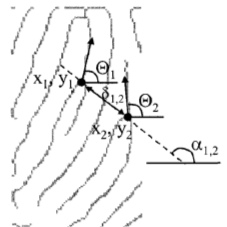
\includegraphics{images/capitulo2/minuciasPuntosCarac.png}
\caption{Puntos característicos tipo bifurcación. Sus coordenadas y orientaciones angulares están dadas por $\left(x_1 , y_1 , \Theta_1 \right)$ y $\left(x_2 , y_2 , \Theta_2 \right)$ .}
\label{minuciasPuntosCarac}
\end{figure}

Hay un gran número de nuevos métodos para la extracción de distancias locales.Independiente de su tipo, la colección de mediciones de distancias locales pueden ser acumuladas durante el proceso de correspondencia, y en consecuencia, dar lugar a una medida de similitud, ya mencionada anteriormente, denominada umbral de decisión, que determina con qué nivel de exactitud queremos verificar o identificar a un sujeto, lo que puede determinar la búsqueda en base a “que tan similar es un sujeto con el patrón almacenado”.


Este método es sólo un ejemplo ilustrativo de cómo tratar un enfoque para características basadas minucias, pero es necesario saber que existe un gran número de enfoques muy distintos al aquí comentado, razón por la que es necesario estudiar literatura adicional para ser más experto en el tema.


\subsection{Identificación por Radio Frecuencia RFID}

Si bien en la actualidad la tecnología más extendida para la identificación de objetos es la de los códigos de barras, éstos presentan algunas desventajas, como son la escasa cantidad de datos que pueden almacenar y la
imposibilidad de ser modificados o reprogramados. La mejora que se ideó, y que constituye el origen de la tecnología RFID, consistía en usar chips de silicio que pudieran transferir los datos que almacenaban al lector sin contacto físico.

Entnces podemos definir RFID como  uns  sistema de  almacenamieto  y  recuperación  de  datos  de  manera remota, utilizando dispositivos denominados tags o etiquetas RFID. El propósito fundamental de la tecnología RFID es transmitir la identidad de un objeto, similar a un número de serie único, mediante ondas de radio.

Un tags RFID es un dispositivo pequeño, similar a una  pegotina, que puede ser adherida en un producto, animal o persona. Contienen antenas para permitir recibir y responder a peticiones por radiofrecuencia desde un emisor-receptor RFID.


Una de las ventajas del uso de radiofrecuencia, en lugar de otras tecnologias como de infrarrojos, es que no se requiere visión directa entre emisor y receptor.

\subsubsection{Arquitectura y tipos de tarjetas}


El funcionamiento de los sistemas RFID es simple. La etiqueta RFID,  genera una señal de radiofrecuencia con la información. Ésta es captada por un lector que lee la información y se la entrega, digitalmente, a la aplicación específica que utiliza RFID.


Por tanto, un sistema RFID consta de tres componentes Etiquetas o Tags RFID, Lector o Transceptor RFID y Aplicación como  se ve en la figura \ref{arqui_RFID}  



\begin{figure}[H]
\centering
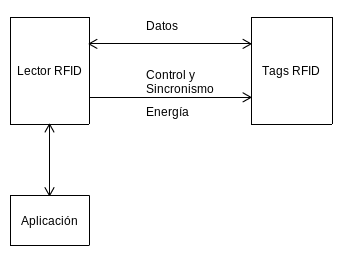
\includegraphics[scale=0.9]{images/capitulo2/arqui_RFID.png}
\caption{Arquitectura de un sistema RFID}
\label{arqui_RFID}
\end{figure}


\myparagraph{Etiqueta RFID}

Esta compuesta por una antena, un radiotransmisor y un material encapsulado o  chip. El propósito de la antena es permitir al chip, que contiene la información, transmitir la información de identificación de la etiqueta. El chip posee una memoria interna con una determinada capacidad, depende del modelo y varía desde una decena hasta millares de bytes.

 Existen varios tipos de memoria:

\begin{itemize}
	\item \textbf{Solo lectura}: El código de identificación que contiene es único y es personalizado durante la fabricación de la etiqueta.

	\item \textbf{De lectura y escritura}: La información de identificación puede ser modificada por el lector.

      	\item \textbf{Anticolisión}: Se trata de etiquetas especiales que permiten que un lector identifique varias al mismo tiempo y no se solapen, normalmente las etiquetas deben ingresar una a una en la zona de cobertura del lector.

\end{itemize}

%-------------------------------------------------------------------------------------------------------------------------------------------



\newpage
%----------------------------------------------------------
%----------------------------------------------------------
\section{SOLUCIÓN PROPUESTA}
%\input{contents/03_Solucion_Propuesta.tex}

\newpage
%----------------------------------------------------------
%----------------------------------------------------------
\section{ANÁLISIS Y DISEÑO}
%\input{contents/04_Analisis_y_Diseno.tex}

\newpage
%----------------------------------------------------------
%----------------------------------------------------------
\section{IMPLEMENTACIÓN}
%\input{contents/05_Implementacion.tex}

\newpage
%----------------------------------------------------------
%----------------------------------------------------------
\section{RESULTADOS}
%\input{contents/06_Resultados.tex}

\newpage
%----------------------------------------------------------
%----------------------------------------------------------
\section{CONCLUSIONES}
%\input{contents/Conclusion.tex}

\newpage
%----------------------------------------------------------
%----------------------------------------------------------


\newpage
%##########################################################
% BIBLIOGRAFIA

\renewcommand{\refname}{BIBLIOGRAFÍA}
\phantomsection
\addcontentsline{toc}{section}{BIBLIOGRAFÍA}
%----------------------------------------------------------
%----------------------------------------------------------
% BIBLIOGRAFÍA

\begin{spacing}{1.0}
\begin{thebibliography}{99}  

\bibitem[Ind09]{Ind09}
Electro Industria. (2009).
\newblock Robótica en Chile. Cada vez más cerca de la automatización total.
\newblock Disponible en \url{http://www.emb.cl/electroindustria/articulo.mvc?xid=1269&tip=9}
\newblock Consultado el 24 de Marzo de 2014.

\bibitem[Osh14]{Osh14}
OSHW-open source hardware. (2014).
\newblock From Definition of Free Cultural Works.
\newblock Disponible en \url{http://freedomdefined.org/OSHW}
\newblock Consultado el 27 de Marzo de 2014.

\bibitem[Del07]{Del07}
Antonio Delgado. (2007).
\newblock ¿Qué es el hardware libre?
\newblock Eroski Consumer
\newblock Disponible en \url{http://www.consumer.es/web/es/tecnologia/hardware/2007/11/20/171514.php}.
\newblock Consultado el 27 de Marzo de 2014.

\bibitem[Car08]{Car08}
Carrasco Livio.  (2008).
\newblock Cancerbero: Prototipo de Control de Acceso utilizando Gestión de espacios mediante Dispositivos Contactless, Smartcard y Biometría.
\newblock Escuela de Ingenieria Civil en Informática
\newblock Universidad Austral  de Chile. 

\bibitem[Vie06]{Vie06}
Vielhauer C. (2006).
\newblock Biometric User Authentication for IT Security: From Fundamentals to Handwriting.
\newblock Springer.

\bibitem[Way00]{Way00}
Wayman J.L. (2000).
\newblock National Biometric Test Center - Collected Works Version 1.2
\newblock Disponible en \url{http://www.engr.sjsu.edu/biometrics/nbtccw.pdf}
\newblock Consultado el 16 de Abril de 2014.


\bibitem[Zha00]{Zha00}
Zhang D. (2000).
\newblock Automated Biometrics, Kluwer
\newblock Springer.


\bibitem[Way99]{Way99}
Wayman J.L. (1999).
\newblock Technical Testing and Evaluation of Biometric Identification Devices.
\newblock Kluwer Academic Publishers.
\newblock Boston, MA, U.S.A, pp. 345 -368


%------------------------------------------------------------------------------------------



\bibitem[Cis11]{Cis11}
Cisco (2011).
\newblock Big Data in the Enterprise: Network Design Considerations.
\newblock Disponible en \url{http://www.cisco.com/en/US/prod/collateral/switches/ps9441/ps9670/white_paper_c11-690561.pdf}.
\newblock Consultado el 20 de Agosto de 2013.

\bibitem[Com09]{Com09}
Commission of the European Communities (2009).
\newblock Internet of Things - An action plan for Europe.
\newblock Disponible en \url{http://eur-lex.europa.eu/LexUriServ/LexUriServ.do?uri=COM:2009:0278:FIN:EN:PDF}.
\newblock Consultado el 01 de Agosto de 2013.

\bibitem[Dee98]{Dee98}
Deering, S. \& Hinden, R. (1998).
\newblock RFC 2460. Internet Protocol, Version 6 (IPv6) Specification. Internet Engineering Task Force.
\newblock Disponible en \url{http://www.ietf.org/rfc/rfc2460.txt}.
\newblock Consultado el 07 de Agosto de 2013.

\bibitem[Del07]{Del07}
Delclós T. (2007).
\newblock El reto del `Internet de las Cosas'. Diario El País.
\newblock Disponible en \url{http://elpais.com/diario/2007/05/17/ciberpais/1179368665_850215.html}.
\newblock Consultado el 01 de Agosto de 2013.

\bibitem[Dun10]{Dun10}
Dunkels A. \& Vasseur JP. (2010).
\newblock White paper \#1: Why IP. IP for Smart Objects.
\newblock Internet Protocol for Smart Objects (IPSO) Alliance.
\newblock Disponible en \url{http://www.ipso-alliance.org/white-papers}.
\newblock Consultado el 06 de Septiembre de 2013.

\bibitem[Els11]{Els11}
Elster Group (2011).
\newblock A Standardized and Flexible IPv6 Architecture for Field Area Networks.
\newblock Smart Grid Last Mile Infrastructure.
\newblock Disponible en \url{http://www.elster.com/assets/downloads/IP-arch-SG-WP-clean-final-112211.pdf}.
\newblock Consultado el 09 de Septiembre de 2013.

\bibitem[Esh]{Esh}
Echaveguren T., Subiabre M., Echaveguren E., \& León C. (n.d.).
\newblock Proposición de un Subsistema de Información para el Sistema de Gestión de Puentes MAPRA.
\newblock Disponible en \url{http://www2.udec.cl/~provial/trabajos_pdf/11TomasEchavegurenSistemapuentesMapra.pdf}.
\newblock Consultado el 07 de Agosto de 2013.

\bibitem[Eur]{Eur}
European Research Cluster on the Internet of Things (n.d.).
\newblock Disponible en \url{http://www.internet-of-things-research.eu/}.
\newblock Consultado el 07 de Agosto de 2013.

\bibitem[Gar09]{Gar09}
Gracía E. (2009).
\newblock Implementación de Protocolos de Transporte en Redes de Sensores.
\newblock Escuela Técnica Superior de Ingeniería de Telecomunicación de Barcelona,
\newblock Universidad Politécnica de Cataluña.

\bibitem[Gut04]{Gut04}
Gutiérrez J., Barrett R. \& Callaway E. (2004).
\newblock Low-rate Wireless Personal Area Networks: Enabling Wireless Sensors with IEEE 802.15.4.
\newblock Institute of Electrical and Electronics Engineers, New York.

\bibitem[Hin06]{Hin06}
Hinden R. \& Deering S. (2006).
\newblock RFC 4291. IP Version 6 Addressing Architecture. Internet Engineering Task Force.
\newblock Disponible en \url{http://www.ietf.org/rfc/rfc4291.txt}.
\newblock Consultado el 07 de Agosto de 2013.

\bibitem[Hui11]{Hui11}
Hui J. \& Thubert P. (2011).
\newblock RFC 6282. Compression Format for IPv6 Datagrams over IEEE 802.15.4-Based Networks. Internet Engineering Task Force.
\newblock Disponible en \url{http://www.ietf.org/rfc/rfc6282.txt}.
\newblock Consultado el 24 de Septiembre de 2013.

\bibitem[IEE03]{IEE03}
IEEE Standards Association (2003).
\newblock IEEE Standard 802.15.4-2003.
\newblock Disponible en \url{http://standards.ieee.org/getieee802/download/802.15.4-2003.pdf}.
\newblock Consultado el 22 de Agosto de 2013.

\bibitem[IMS12]{IMS12}
IMS Research (2012).
\newblock Internet Connected Devices Approaching 10 Billion, to exceed 28 Billion by 2020.
\newblock Disponible en \url{http://www.imsresearch.com/press-release/Internet_Connected_Devices_Approaching_10_Billion_to_exceed_28_Billion_by_2020}.
\newblock Consultado el 28 de Agosto de 2013.

\bibitem[IPv11]{IPv11}
IPv6 para Chile (2011).
\newblock Fase de Inteligencia de Mercados y Competitiva. Informe de Tendencias N$^{o}$ 6.
\newblock Disponible en \url{http://www.ipv6.cl/system/files/Informe-de-Tendencias-enero-2011.pdf}.
\newblock Consultado el 09 de Septiembre de 2013.

\bibitem[Jim12]{Jim12}
Jiménez A., Jiménez S., Lozada P. \& Jiménez C. (2012).
\newblock Wireless Sensors Network in the Efficient Management of Greenhouse Crops.
\newblock 2012 Ninth International Conference on Information Technology - New Generations.
\newblock Las Vegas, 680 - 685. 

\bibitem[Kas13]{Kas13}
Kaschel H. \& Iturralde D. (2013).
\newblock Análisis de Mejoras en la Agricultura Aplicando WSN: Cultivo de Rosas.
\newblock XIV Congreso Internacional de Telecomunicaciones SENACITEL 2013,
\newblock Valdivia. 

\bibitem[Kuo07]{Kuo07}
Kuorilehto M., Kohvakka M., Suhonen J., Hämäläinen P., Hännikäinen M. \& Hämäläinen TD. (2007).
\newblock Ultra-Low Energy Wireless Sensor Networks in Practice.
\newblock Wiley, Great Britain.

\bibitem[Kus07]{Kus07}
Kushalnagar N., Montenegro G. \& Schumacher C. (2007).
\newblock RFC 4919. IPv6 over Low-Power Wireless Personal Area Networks (6LoWPANs): Overview, Assumptions, Problem Statement, and Goals. Internet Engineering Task Force.
\newblock Disponible en \url{http://www.ietf.org/rfc/rfc4919.txt}.
\newblock Consultado el 07 de Agosto de 2013.

\bibitem[Lar99]{Lar99}
Larman C. (1999).
\newblock UML y Patrones: Introducción Al Análisis y Diseño Orientado a Objetos.
\newblock Prentice-Hall, México.

\bibitem[Lat12]{Lat12}
Latin America and Caribbean Network Information Centre (2012).
\newblock Estado de IPv4 a fin de 2012.
\newblock Disponible en: \url{http://portalipv6.lacnic.net/estado-de-ipv4-a-fin-de-2012-es/}.
\newblock Consultado el 20 de Agosto de 2013.

\bibitem[Max06]{Max06}
MaxStream (2006).
\newblock XBee$^{TM}$/XBee-PRO$^{TM}$ OEM RF Modules. Product Manual v1.xAx - 802.15.4 Protocol.
\newblock MaxStream, Inc., London.

\bibitem[Mol12]{Mol12}
Molina N. (2012).
\newblock Diseño de un Sistema de Gestión de Puentes bajo Enfoque de Priorización de la Inversión.
\newblock Escuela de Ingeniería Civil en Obras Civiles,
\newblock Universidad Austral de Chile, Valdivia.

\bibitem[Mon07]{Mon07}
Montenegro G., Kushalnagar N., Hui J. \& Culler D. (2007).
\newblock RFC 4944. Transmission of IPv6 Packets over IEEE 802.15.4 Networks. Internet Engineering Task Force.
\newblock Disponible en \url{http://www.ietf.org/rfc/rfc4944.txt}.
\newblock Consultado el 07 de Agosto de 2013.

\bibitem[Nar07]{Nar07}
Narten T., Nordmark E., Simpson W. \& Soliman H. (2007).
\newblock RFC 4861. Neighbor Discovery for IP version 6 (IPv6). Internet Engineering Task Force.
\newblock Disponible en \url{http://www.ietf.org/rfc/rfc4861.txt}.
\newblock Consultado el 07 de Agosto de 2013.

\bibitem[Nat10]{Nat10}
National Institute of Standards and Technology (2010).
\newblock NIST Framework and Roadmap for Smart Grid Interoperability Standards, Release 1.0.
\newblock Disponible en \url{http://www.nist.gov/public_affairs/releases/upload/smartgrid_interoperability_final.pdf}.
\newblock Consultado el 09 de Septiembre de 2013.

\bibitem[NXP11]{NXP11}
NXP Laboratories UK  Ltd  (2011). 
\newblock JenNet-IP Network Protocol Stack. Low-Power Wireless IP Networking for the `Internet of Things'.
\newblock Disponible en \url{http://www.jennic.com/files/product_briefs/JenNet-IP-PBv1.2docx.pdf}.
\newblock Consultado el 01 de Agosto de 2013.

\bibitem[Och]{Och}
Ochoa A. (n.d.).
\newblock Métodos científicos.
\newblock Disponible en \url{http://www.monografias.com/trabajos11/metods/metods.shtml}.
\newblock Consultado el 23 de Septiembre de 2013.

\bibitem[Oya10]{Oya10}
Oyarce A. (2010).
\newblock Guía del Usuario XBEE Series 1.
\newblock Ingeniería MCI Ltda., Santiago.

\bibitem[Peñ13]{Peñ13}
Peña C. \& Ralli C. (2013).
\newblock IPv6: El motor de ``La WEB de las Cosas''. Blog Think Big.
\newblock Disponible en \url{http://blogthinkbig.com/ipv6-motor-internet-de-las-cosas-iot/}.
\newblock Consultado el 27 de Agosto de 2013.

\bibitem[Pos80]{Pos80}
Postel J. (1980).
\newblock RFC 768. User Datagram Protocol. Internet Engineering Task Force.
\newblock Disponible en \url{http://www.ietf.org/rfc/rfc768.txt}.
\newblock Consultado el 06 de Septiembre de 2013.

\bibitem[Rev09]{Rev09}
Reventós  L. (2009).
\newblock El `Internet de las Cosas' ahorraría 200000 muertes anuales en las carreteras europeas. Diario El País, Tecnología.
\newblock Disponible en \url{http://tecnologia.elpais.com/tecnologia/2009/05/20/actualidad/1242810061_850215.html}.
\newblock Consultado el 01 de Agosto de 2013.

\bibitem[Rya01]{Rya01}
Ryall M. (2001).
\newblock Bridge Management.
\newblock Elsevier, Great Britain.

\bibitem[Scr13]{Scr13}
Scrum Manager (2013).
\newblock Scrum Manager BoK (SMBoK).
\newblock Disponible en: \url{http://www.scrummanager.net/bok/index.php?title=Main_Page}.
\newblock Consultado el 25 de Septiembre de 2013.

\bibitem[She09]{She09}
Shelby Z. \& Bormann C. (2009).
\newblock 6LoWPAN: The Wireless Embedded Internet.
\newblock Wiley, Great Britain.

\bibitem[She12]{She12}
Shelby Z., Chakrabarti S., Nordmark E. \& Bormann C. (2012).
\newblock RFC 6775. Neighbor Discovery Optimization for IPv6 over Low-Power Wireless Personal Area Networks (6LoWPANs). Internet Engineering Task Force.
\newblock Disponible en \url{http://www.ietf.org/rfc/rfc6775.txt}.
\newblock Consultado el 24 de Septiembre de 2013.

\bibitem[She13]{She13}
Shelby Z., Hartke K. \& Bormann C. (2013).
\newblock draft-ietf-core-coap-18. Constrained Application Protocol (CoAP). Internet Engineering Task Force.
\newblock Disponible en \url{http://tools.ietf.org/id/draft-ietf-core-coap-18.txt}.
\newblock Consultado el 01 de Octubre de 2013.

\bibitem[Taf12]{Taf12}
Taffernaberry  C. (2012).
\newblock 6LoWPAN: IPv6 for Wireless Sensor Network.
\newblock Simposio Argentino de Sistemas Embebidos (SASE).
\newblock Disponible en \url{http://www.sase.com.ar/2012/files/2012/09/4-2012-SASE-6lowpan.pdf}.
\newblock Consultado el 21 de Agosto de 2013. 

\bibitem[Tel13]{Tel13}
Telecom Bretagne (2013).
\newblock Arduino $\mu$IPv6 Stack.
\newblock Disponible en \url{https://github.com/telecombretagne/Arduino-IPv6Stack/wiki}.
\newblock Consultado el 24 de Septiembre de 2013. 

\bibitem[Win12]{Win12}
Winter T., Thubert P., Brandt A., Hui J., Kelsey R., Levis P., Pister K., Struik R., Vasseur JP \& Alexander R. (2012). 
\newblock RFC 6550. RPL: IPv6 Routing Protocol for Low-Power and Lossy Networks . Internet Engineering Task Force.
\newblock Available: \url{http://www.ietf.org/rfc/rfc6550.txt}.
\newblock Consultado el 29 de Agosto de 2013.

\bibitem[Yu06]{Yu06}
Yu Y., Prasanna VK., \& Krishnamachari B. (2006).
\newblock Information Processing and Routing in Wireless Sensor Networks.
\newblock World Scientific Publishing Co. Pte. Ltd., Singapore.

\bibitem[Zia08]{Zia08}
Ziadé T. (2008).
\newblock Expert Python Programming. Best practices for designing, coding, and distributing your Python software.
\newblock Packt Publishing, Birmingham.

\end{thebibliography}	
\end{spacing}

%----------------------------------------------------------
%----------------------------------------------------------



	
\newpage
%##########################################################
% ANEXOS

\phantomsection
\addcontentsline{toc}{section}{ANEXOS}

\newpage
%%----------------------------------------------------------
%----------------------------------------------------------
% Anexo E: Lista de abreviaciones
\subsection*{Anexo E: Lista de abreviaciones}
\addcontentsline{toc}{subsection}{Anexo E: Lista de abreviaciones}
\label{anexo-e}

\vspace{0.5cm}

\begin{spacing}{1.2}
\textbf{6LoWPAN:} IPv6 over Low-Power Wireless Personal Area Networks\\
\textbf{ACID:} Atomicity, Consistency, Isolation, Durability\\ 
\textbf{API:} Application Programming Interface\\
\textbf{BLIP:} Berkeley IP Implementation\\
\textbf{BMS:} Bridge Management System\\
\textbf{CoAP:} Constrained Application Protocol\\
\textbf{CPU:} Central Processing Unit\\
\textbf{DC:} Corriente directa (direct current)\\
\textbf{DIN:} Deutsches Institut für Normung\\
\textbf{FAN:} Field Area Network\\
\textbf{FCS:} Frame Check Sequence\\
\textbf{HTML:} HyperText Markup Language\\
\textbf{HTTP:} Hypertext Transfer Protocol\\
\textbf{ICMP:} Internet Control Message Protocol\\
\textbf{IDE:} Integrated Development Environment\\
\textbf{IEEE:} Institute of Electrical and Electronics Engineers\\
\textbf{IERC:} European Research Cluster on the Internet of Things\\
\textbf{IETF:} Internet Engineering Task Force\\
\textbf{IID:} Interface IDentifier\\
\textbf{IoT:} Internet of Things\\
\textbf{IP:} Internet Protocol\\
\textbf{IPv4:} Internet Protocol version 4\\
\textbf{IPv6:} Internet Protocol version 6\\
\textbf{IPSO:} IP for Smart Objects (Alliance)\\
\textbf{ISA:} International Society of Automation\\
\textbf{ISM:} Industrial, Scientific and Medical\\
\textbf{JSON:} JavaScript Object Notation\\
\textbf{LACNIC:} Latin America and Caribbean Network Information Centre\\
\textbf{LAMP:} Linux, Apache, MySQL, PHP\\
\textbf{LLN:} Low power and Lossy Networks\\
\textbf{LoWPAN:} Low-Power Wireless Area Network\\
\textbf{LR-WPAN:} Low-rate Wireless Personal Area Network\\
\textbf{MAC:} Media Access Control layer\\ 
\textbf{MAPRA:} Mantenimiento de Puentes de la Red Vial Austral\\
\textbf{MIT:} Massachusetts Institute of Technology\\
\textbf{MOP:} Ministerio de Obras Públicas\\
\textbf{NIST:} National Institute of Standards and Technology\\
\textbf{ND:} Neighbor Discovery\\
\textbf{OECD:} Organisation for Economic Co-operation and Development\\
\textbf{OS:} Operating System\\
\textbf{OSI:} Open System Interconnection\\
\textbf{PHY:} Physical layer\\
\textbf{POS:} Point Of Service\\
\textbf{RFC:} Request for Comments\\
\textbf{RFID:} Radio Frequency IDentification\\
\textbf{ROLL:} Routing over Low-power and Lossy Networks\\
\textbf{RPL:} Ripple routing protocol\\
\textbf{RSSI:} Received Signal Strength Indicator\\
\textbf{SBC:} Single Board Computer\\
\textbf{SICS:} Swedish Institute for Computer Science\\
\textbf{SNAP:} Simple Network Access Protocol\\
\textbf{SNMP:} Simple Network Management Protocol\\
\textbf{TCP:} Transmission Control Protocol\\
\textbf{UACh:} Universidad Austral de Chile\\
\textbf{UART:} Universal Asynchronous Receiver-Transmitter\\
\textbf{UDP:} User Datagram Protocol\\
\textbf{UI:} User Interface\\
\textbf{UML:} Unified Modeling Language\\
\textbf{WAN:} Wide Area Network\\
\textbf{WHAN:} Wireless Home Area Network\\
\textbf{WLAN:} Wireless Local Area Network\\
\textbf{WMAN:} Wireless Metropolitan Area Network\\
\textbf{WPAN:} Wireless Personal Area Network\\
\textbf{WSN:} Wireless Sensor Network\\
\textbf{WWAN:} Wireless Wide Area Network\\
\textbf{XML:} eXtensible Markup Language\\
\end{spacing}


%----------------------------------------------------------
%----------------------------------------------------------


\end{document} 
